% Options for packages loaded elsewhere
\PassOptionsToPackage{unicode}{hyperref}
\PassOptionsToPackage{hyphens}{url}
\PassOptionsToPackage{dvipsnames,svgnames,x11names}{xcolor}
%
\documentclass[
  letterpaper,
  DIV=11,
  numbers=noendperiod]{scrartcl}

\usepackage{amsmath,amssymb}
\usepackage{iftex}
\ifPDFTeX
  \usepackage[T1]{fontenc}
  \usepackage[utf8]{inputenc}
  \usepackage{textcomp} % provide euro and other symbols
\else % if luatex or xetex
  \usepackage{unicode-math}
  \defaultfontfeatures{Scale=MatchLowercase}
  \defaultfontfeatures[\rmfamily]{Ligatures=TeX,Scale=1}
\fi
\usepackage{lmodern}
\ifPDFTeX\else  
    % xetex/luatex font selection
\fi
% Use upquote if available, for straight quotes in verbatim environments
\IfFileExists{upquote.sty}{\usepackage{upquote}}{}
\IfFileExists{microtype.sty}{% use microtype if available
  \usepackage[]{microtype}
  \UseMicrotypeSet[protrusion]{basicmath} % disable protrusion for tt fonts
}{}
\makeatletter
\@ifundefined{KOMAClassName}{% if non-KOMA class
  \IfFileExists{parskip.sty}{%
    \usepackage{parskip}
  }{% else
    \setlength{\parindent}{0pt}
    \setlength{\parskip}{6pt plus 2pt minus 1pt}}
}{% if KOMA class
  \KOMAoptions{parskip=half}}
\makeatother
\usepackage{xcolor}
\setlength{\emergencystretch}{3em} % prevent overfull lines
\setcounter{secnumdepth}{5}
% Make \paragraph and \subparagraph free-standing
\ifx\paragraph\undefined\else
  \let\oldparagraph\paragraph
  \renewcommand{\paragraph}[1]{\oldparagraph{#1}\mbox{}}
\fi
\ifx\subparagraph\undefined\else
  \let\oldsubparagraph\subparagraph
  \renewcommand{\subparagraph}[1]{\oldsubparagraph{#1}\mbox{}}
\fi

\usepackage{color}
\usepackage{fancyvrb}
\newcommand{\VerbBar}{|}
\newcommand{\VERB}{\Verb[commandchars=\\\{\}]}
\DefineVerbatimEnvironment{Highlighting}{Verbatim}{commandchars=\\\{\}}
% Add ',fontsize=\small' for more characters per line
\usepackage{framed}
\definecolor{shadecolor}{RGB}{241,243,245}
\newenvironment{Shaded}{\begin{snugshade}}{\end{snugshade}}
\newcommand{\AlertTok}[1]{\textcolor[rgb]{0.68,0.00,0.00}{#1}}
\newcommand{\AnnotationTok}[1]{\textcolor[rgb]{0.37,0.37,0.37}{#1}}
\newcommand{\AttributeTok}[1]{\textcolor[rgb]{0.40,0.45,0.13}{#1}}
\newcommand{\BaseNTok}[1]{\textcolor[rgb]{0.68,0.00,0.00}{#1}}
\newcommand{\BuiltInTok}[1]{\textcolor[rgb]{0.00,0.23,0.31}{#1}}
\newcommand{\CharTok}[1]{\textcolor[rgb]{0.13,0.47,0.30}{#1}}
\newcommand{\CommentTok}[1]{\textcolor[rgb]{0.37,0.37,0.37}{#1}}
\newcommand{\CommentVarTok}[1]{\textcolor[rgb]{0.37,0.37,0.37}{\textit{#1}}}
\newcommand{\ConstantTok}[1]{\textcolor[rgb]{0.56,0.35,0.01}{#1}}
\newcommand{\ControlFlowTok}[1]{\textcolor[rgb]{0.00,0.23,0.31}{#1}}
\newcommand{\DataTypeTok}[1]{\textcolor[rgb]{0.68,0.00,0.00}{#1}}
\newcommand{\DecValTok}[1]{\textcolor[rgb]{0.68,0.00,0.00}{#1}}
\newcommand{\DocumentationTok}[1]{\textcolor[rgb]{0.37,0.37,0.37}{\textit{#1}}}
\newcommand{\ErrorTok}[1]{\textcolor[rgb]{0.68,0.00,0.00}{#1}}
\newcommand{\ExtensionTok}[1]{\textcolor[rgb]{0.00,0.23,0.31}{#1}}
\newcommand{\FloatTok}[1]{\textcolor[rgb]{0.68,0.00,0.00}{#1}}
\newcommand{\FunctionTok}[1]{\textcolor[rgb]{0.28,0.35,0.67}{#1}}
\newcommand{\ImportTok}[1]{\textcolor[rgb]{0.00,0.46,0.62}{#1}}
\newcommand{\InformationTok}[1]{\textcolor[rgb]{0.37,0.37,0.37}{#1}}
\newcommand{\KeywordTok}[1]{\textcolor[rgb]{0.00,0.23,0.31}{#1}}
\newcommand{\NormalTok}[1]{\textcolor[rgb]{0.00,0.23,0.31}{#1}}
\newcommand{\OperatorTok}[1]{\textcolor[rgb]{0.37,0.37,0.37}{#1}}
\newcommand{\OtherTok}[1]{\textcolor[rgb]{0.00,0.23,0.31}{#1}}
\newcommand{\PreprocessorTok}[1]{\textcolor[rgb]{0.68,0.00,0.00}{#1}}
\newcommand{\RegionMarkerTok}[1]{\textcolor[rgb]{0.00,0.23,0.31}{#1}}
\newcommand{\SpecialCharTok}[1]{\textcolor[rgb]{0.37,0.37,0.37}{#1}}
\newcommand{\SpecialStringTok}[1]{\textcolor[rgb]{0.13,0.47,0.30}{#1}}
\newcommand{\StringTok}[1]{\textcolor[rgb]{0.13,0.47,0.30}{#1}}
\newcommand{\VariableTok}[1]{\textcolor[rgb]{0.07,0.07,0.07}{#1}}
\newcommand{\VerbatimStringTok}[1]{\textcolor[rgb]{0.13,0.47,0.30}{#1}}
\newcommand{\WarningTok}[1]{\textcolor[rgb]{0.37,0.37,0.37}{\textit{#1}}}

\providecommand{\tightlist}{%
  \setlength{\itemsep}{0pt}\setlength{\parskip}{0pt}}\usepackage{longtable,booktabs,array}
\usepackage{calc} % for calculating minipage widths
% Correct order of tables after \paragraph or \subparagraph
\usepackage{etoolbox}
\makeatletter
\patchcmd\longtable{\par}{\if@noskipsec\mbox{}\fi\par}{}{}
\makeatother
% Allow footnotes in longtable head/foot
\IfFileExists{footnotehyper.sty}{\usepackage{footnotehyper}}{\usepackage{footnote}}
\makesavenoteenv{longtable}
\usepackage{graphicx}
\makeatletter
\def\maxwidth{\ifdim\Gin@nat@width>\linewidth\linewidth\else\Gin@nat@width\fi}
\def\maxheight{\ifdim\Gin@nat@height>\textheight\textheight\else\Gin@nat@height\fi}
\makeatother
% Scale images if necessary, so that they will not overflow the page
% margins by default, and it is still possible to overwrite the defaults
% using explicit options in \includegraphics[width, height, ...]{}
\setkeys{Gin}{width=\maxwidth,height=\maxheight,keepaspectratio}
% Set default figure placement to htbp
\makeatletter
\def\fps@figure{htbp}
\makeatother

\KOMAoption{captions}{tableheading}
\makeatletter
\makeatother
\makeatletter
\makeatother
\makeatletter
\@ifpackageloaded{caption}{}{\usepackage{caption}}
\AtBeginDocument{%
\ifdefined\contentsname
  \renewcommand*\contentsname{Table of contents}
\else
  \newcommand\contentsname{Table of contents}
\fi
\ifdefined\listfigurename
  \renewcommand*\listfigurename{List of Figures}
\else
  \newcommand\listfigurename{List of Figures}
\fi
\ifdefined\listtablename
  \renewcommand*\listtablename{List of Tables}
\else
  \newcommand\listtablename{List of Tables}
\fi
\ifdefined\figurename
  \renewcommand*\figurename{Figure}
\else
  \newcommand\figurename{Figure}
\fi
\ifdefined\tablename
  \renewcommand*\tablename{Table}
\else
  \newcommand\tablename{Table}
\fi
}
\@ifpackageloaded{float}{}{\usepackage{float}}
\floatstyle{ruled}
\@ifundefined{c@chapter}{\newfloat{codelisting}{h}{lop}}{\newfloat{codelisting}{h}{lop}[chapter]}
\floatname{codelisting}{Listing}
\newcommand*\listoflistings{\listof{codelisting}{List of Listings}}
\makeatother
\makeatletter
\@ifpackageloaded{caption}{}{\usepackage{caption}}
\@ifpackageloaded{subcaption}{}{\usepackage{subcaption}}
\makeatother
\makeatletter
\@ifpackageloaded{tcolorbox}{}{\usepackage[skins,breakable]{tcolorbox}}
\makeatother
\makeatletter
\@ifundefined{shadecolor}{\definecolor{shadecolor}{rgb}{.97, .97, .97}}
\makeatother
\makeatletter
\makeatother
\makeatletter
\makeatother
\ifLuaTeX
  \usepackage{selnolig}  % disable illegal ligatures
\fi
\IfFileExists{bookmark.sty}{\usepackage{bookmark}}{\usepackage{hyperref}}
\IfFileExists{xurl.sty}{\usepackage{xurl}}{} % add URL line breaks if available
\urlstyle{same} % disable monospaced font for URLs
\hypersetup{
  pdftitle={Bootstrapping and Confidence Intervals},
  pdfauthor={Justin Baumann},
  colorlinks=true,
  linkcolor={blue},
  filecolor={Maroon},
  citecolor={Blue},
  urlcolor={Blue},
  pdfcreator={LaTeX via pandoc}}

\title{Bootstrapping and Confidence Intervals}
\author{Justin Baumann}
\date{}

\begin{document}
\maketitle
\ifdefined\Shaded\renewenvironment{Shaded}{\begin{tcolorbox}[frame hidden, sharp corners, interior hidden, boxrule=0pt, breakable, borderline west={3pt}{0pt}{shadecolor}, enhanced]}{\end{tcolorbox}}\fi

\renewcommand*\contentsname{Table of contents}
{
\hypersetup{linkcolor=}
\setcounter{tocdepth}{3}
\tableofcontents
}
\hypertarget{bootstrapping-and-eventually-confidence-intervals}{%
\section{\texorpdfstring{\textbf{Bootstrapping (and eventually
confidence
intervals)}}{Bootstrapping (and eventually confidence intervals)}}\label{bootstrapping-and-eventually-confidence-intervals}}

\hypertarget{resources}{%
\section{Resources}\label{resources}}

\href{https://moderndive.com/8-confidence-intervals.html}{Smith College
SDS CIs tutorial}\\
\href{https://mdsr-book.github.io/mdsr2e/ch-foundations.html\#sec:boot}{Modern
Data Science with R text chapter}

\hypertarget{load-packages}{%
\section{Load Packages}\label{load-packages}}

\begin{Shaded}
\begin{Highlighting}[]
\FunctionTok{library}\NormalTok{(tidyverse)}
\FunctionTok{library}\NormalTok{(palmerpenguins)}
\FunctionTok{library}\NormalTok{(data.table)}
\FunctionTok{library}\NormalTok{(performance)}
\FunctionTok{library}\NormalTok{(patchwork)}
\FunctionTok{library}\NormalTok{(rsample) }\CommentTok{\#for lm bootstraps}
\FunctionTok{library}\NormalTok{(car) }\CommentTok{\#to check collinearity}
\FunctionTok{library}\NormalTok{(skimr)}
\FunctionTok{library}\NormalTok{(broom)}
\end{Highlighting}
\end{Shaded}

\hypertarget{get-penguins-data}{%
\section{Get Penguins data!}\label{get-penguins-data}}

\begin{Shaded}
\begin{Highlighting}[]
\NormalTok{penguins}\OtherTok{\textless{}{-}}\NormalTok{palmerpenguins}\SpecialCharTok{::}\NormalTok{penguins}
\end{Highlighting}
\end{Shaded}

\hypertarget{fit-a-simple-lm-and-have-a-look-at-results}{%
\section{Fit a simple LM and have a look at
results}\label{fit-a-simple-lm-and-have-a-look-at-results}}

\begin{Shaded}
\begin{Highlighting}[]
\NormalTok{simple\_mod}\OtherTok{\textless{}{-}}\FunctionTok{lm}\NormalTok{(bill\_depth\_mm }\SpecialCharTok{\textasciitilde{}}\NormalTok{ bill\_length\_mm}\SpecialCharTok{*}\NormalTok{species}\SpecialCharTok{*}\NormalTok{sex, }\AttributeTok{data=}\NormalTok{penguins)}

\FunctionTok{summary}\NormalTok{(simple\_mod)}
\end{Highlighting}
\end{Shaded}

\begin{verbatim}

Call:
lm(formula = bill_depth_mm ~ bill_length_mm * species * sex, 
    data = penguins)

Residuals:
     Min       1Q   Median       3Q      Max 
-2.06730 -0.52452 -0.06471  0.45593  2.90319 

Coefficients:
                                         Estimate Std. Error t value Pr(>|t|)
(Intercept)                              14.84023    1.77185   8.376 1.73e-15
bill_length_mm                            0.07466    0.04749   1.572   0.1169
speciesChinstrap                         -0.25160    2.77579  -0.091   0.9278
speciesGentoo                            -5.76780    2.98938  -1.929   0.0546
sexmale                                   4.92359    2.46355   1.999   0.0465
bill_length_mm:speciesChinstrap          -0.01026    0.06596  -0.155   0.8765
bill_length_mm:speciesGentoo              0.03871    0.07101   0.545   0.5860
bill_length_mm:sexmale                   -0.09177    0.06360  -1.443   0.1500
speciesChinstrap:sexmale                -11.35403    5.67926  -1.999   0.0464
speciesGentoo:sexmale                    -2.41202    3.94469  -0.611   0.5413
bill_length_mm:speciesChinstrap:sexmale   0.24451    0.12006   2.037   0.0425
bill_length_mm:speciesGentoo:sexmale      0.06197    0.09131   0.679   0.4978
                                           
(Intercept)                             ***
bill_length_mm                             
speciesChinstrap                           
speciesGentoo                           .  
sexmale                                 *  
bill_length_mm:speciesChinstrap            
bill_length_mm:speciesGentoo               
bill_length_mm:sexmale                     
speciesChinstrap:sexmale                *  
speciesGentoo:sexmale                      
bill_length_mm:speciesChinstrap:sexmale *  
bill_length_mm:speciesGentoo:sexmale       
---
Signif. codes:  0 '***' 0.001 '**' 0.01 '*' 0.05 '.' 0.1 ' ' 1

Residual standard error: 0.8175 on 321 degrees of freedom
  (11 observations deleted due to missingness)
Multiple R-squared:  0.8334,    Adjusted R-squared:  0.8277 
F-statistic: 145.9 on 11 and 321 DF,  p-value: < 2.2e-16
\end{verbatim}

\begin{Shaded}
\begin{Highlighting}[]
\NormalTok{broom}\SpecialCharTok{::}\FunctionTok{tidy}\NormalTok{(simple\_mod)}
\end{Highlighting}
\end{Shaded}

\begin{verbatim}
# A tibble: 12 x 5
   term                                    estimate std.error statistic  p.value
   <chr>                                      <dbl>     <dbl>     <dbl>    <dbl>
 1 (Intercept)                              14.8       1.77      8.38   1.73e-15
 2 bill_length_mm                            0.0747    0.0475    1.57   1.17e- 1
 3 speciesChinstrap                         -0.252     2.78     -0.0906 9.28e- 1
 4 speciesGentoo                            -5.77      2.99     -1.93   5.46e- 2
 5 sexmale                                   4.92      2.46      2.00   4.65e- 2
 6 bill_length_mm:speciesChinstrap          -0.0103    0.0660   -0.155  8.77e- 1
 7 bill_length_mm:speciesGentoo              0.0387    0.0710    0.545  5.86e- 1
 8 bill_length_mm:sexmale                   -0.0918    0.0636   -1.44   1.50e- 1
 9 speciesChinstrap:sexmale                -11.4       5.68     -2.00   4.64e- 2
10 speciesGentoo:sexmale                    -2.41      3.94     -0.611  5.41e- 1
11 bill_length_mm:speciesChinstrap:sexmale   0.245     0.120     2.04   4.25e- 2
12 bill_length_mm:speciesGentoo:sexmale      0.0620    0.0913    0.679  4.98e- 1
\end{verbatim}

\hypertarget{now-lets-bootstrap}{%
\section{Now, let's bootstrap!}\label{now-lets-bootstrap}}

Bootstrapping is a resampling technique. We will discuss how it works!

\begin{Shaded}
\begin{Highlighting}[]
\FunctionTok{set.seed}\NormalTok{(}\DecValTok{356}\NormalTok{) }\CommentTok{\#any number is fine}

\NormalTok{penguins\_intervals}\OtherTok{\textless{}{-}} \FunctionTok{reg\_intervals}\NormalTok{(bill\_depth\_mm }\SpecialCharTok{\textasciitilde{}}\NormalTok{ bill\_length\_mm}\SpecialCharTok{*}\NormalTok{species}\SpecialCharTok{*}\NormalTok{sex, }\AttributeTok{data=}\NormalTok{penguins, }
                                   \AttributeTok{type=}\StringTok{\textquotesingle{}percentile\textquotesingle{}}\NormalTok{,}
                                   \AttributeTok{keep\_reps=}\ConstantTok{FALSE}\NormalTok{)}

\NormalTok{penguins\_intervals}
\end{Highlighting}
\end{Shaded}

\begin{verbatim}
# A tibble: 11 x 6
   term                                  .lower .estimate  .upper .alpha .method
   <chr>                                  <dbl>     <dbl>   <dbl>  <dbl> <chr>  
 1 bill_length_mm                       -0.0441   0.0722   0.188    0.05 percen~
 2 bill_length_mm:sexmale               -0.264   -0.0907   0.0827   0.05 percen~
 3 bill_length_mm:speciesChinstrap      -0.138   -0.00259  0.135    0.05 percen~
 4 bill_length_mm:speciesChinstrap:se~  -0.0130   0.239    0.495    0.05 percen~
 5 bill_length_mm:speciesGentoo         -0.0959   0.0401   0.171    0.05 percen~
 6 bill_length_mm:speciesGentoo:sexma~  -0.141    0.0598   0.266    0.05 percen~
 7 sexmale                              -1.93     4.87    11.6      0.05 percen~
 8 speciesChinstrap                     -6.21    -0.584    4.73     0.05 percen~
 9 speciesChinstrap:sexmale            -23.0    -11.1      0.527    0.05 percen~
10 speciesGentoo                       -11.0     -5.82    -0.426    0.05 percen~
11 speciesGentoo:sexmale               -10.8     -2.30     6.08     0.05 percen~
\end{verbatim}

\begin{Shaded}
\begin{Highlighting}[]
\CommentTok{\#plot the results}
\NormalTok{penboots}\OtherTok{\textless{}{-}}\FunctionTok{ggplot}\NormalTok{(}\AttributeTok{data=}\NormalTok{penguins\_intervals, }\FunctionTok{aes}\NormalTok{(}\AttributeTok{x=}\NormalTok{.estimate, }\AttributeTok{y=}\NormalTok{term))}\SpecialCharTok{+}
  \FunctionTok{geom\_vline}\NormalTok{(}\AttributeTok{xintercept=}\DecValTok{0}\NormalTok{, }\AttributeTok{linetype=}\DecValTok{2}\NormalTok{)}\SpecialCharTok{+}
  \FunctionTok{geom\_errorbarh}\NormalTok{(}\FunctionTok{aes}\NormalTok{(}\AttributeTok{xmin=}\NormalTok{.lower, }\AttributeTok{xmax=}\NormalTok{.upper),}\AttributeTok{height=}\FloatTok{0.2}\NormalTok{)}\SpecialCharTok{+}
  \FunctionTok{geom\_point}\NormalTok{(}\AttributeTok{size=}\DecValTok{3}\NormalTok{)}\SpecialCharTok{+}
  \FunctionTok{theme\_classic}\NormalTok{()}
\NormalTok{penboots}
\end{Highlighting}
\end{Shaded}

\begin{figure}[H]

{\centering 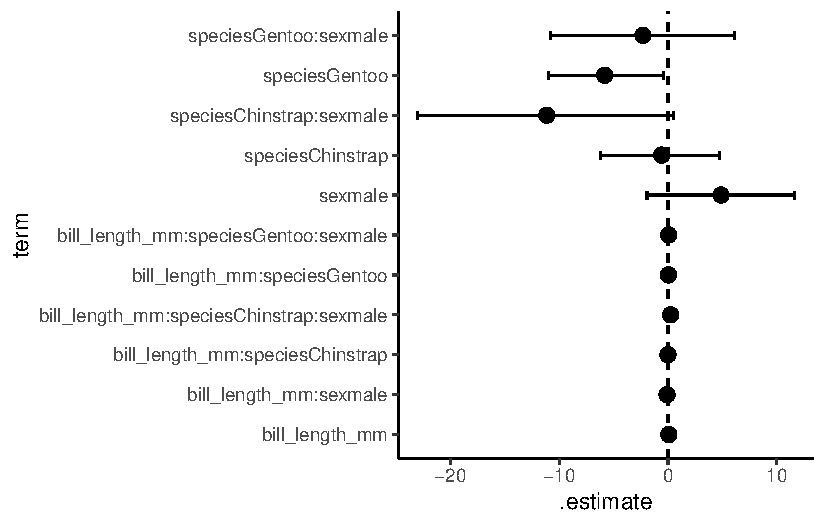
\includegraphics{CIs_files/figure-pdf/unnamed-chunk-4-1.pdf}

}

\end{figure}

\hypertarget{understanding-resampling-and-bootstrapping-using-tidyverse}{%
\section{\texorpdfstring{\textbf{Understanding resampling and
bootstrapping using
tidyverse}}{Understanding resampling and bootstrapping using tidyverse}}\label{understanding-resampling-and-bootstrapping-using-tidyverse}}

\hypertarget{lets-take-a-sample-of-the-penguins-data}{%
\subsection{Let's take a sample of the penguins
data}\label{lets-take-a-sample-of-the-penguins-data}}

\begin{Shaded}
\begin{Highlighting}[]
\NormalTok{lilpen}\OtherTok{\textless{}{-}}\NormalTok{ penguins }\SpecialCharTok{\%\textgreater{}\%}
  \FunctionTok{slice\_sample}\NormalTok{(}\AttributeTok{n=}\DecValTok{10}\NormalTok{, }\AttributeTok{replace=} \ConstantTok{FALSE}\NormalTok{) }\SpecialCharTok{\%\textgreater{}\%}
  \FunctionTok{select}\NormalTok{(species, sex, year, bill\_length\_mm)}

\NormalTok{lilpen}
\end{Highlighting}
\end{Shaded}

\begin{verbatim}
# A tibble: 10 x 4
   species   sex     year bill_length_mm
   <fct>     <fct>  <int>          <dbl>
 1 Gentoo    female  2007           48.7
 2 Adelie    male    2008           39.6
 3 Gentoo    female  2009           50.5
 4 Adelie    female  2007           40.3
 5 Gentoo    male    2008           44.4
 6 Adelie    female  2009           40.2
 7 Gentoo    female  2007           46.2
 8 Gentoo    female  2007           45.1
 9 Chinstrap female  2007           58  
10 Gentoo    male    2009           52.5
\end{verbatim}

\begin{Shaded}
\begin{Highlighting}[]
\CommentTok{\#let\textquotesingle{}s turn resampling on (let\textquotesingle{}s us include duplicates{-}{-} we can choose from entire dataset AGAIN when we collect a separate sample)}
\NormalTok{lilpen2}\OtherTok{\textless{}{-}}\NormalTok{ penguins }\SpecialCharTok{\%\textgreater{}\%}
  \FunctionTok{slice\_sample}\NormalTok{(}\AttributeTok{n=}\DecValTok{10}\NormalTok{, }\AttributeTok{replace=} \ConstantTok{TRUE}\NormalTok{) }\SpecialCharTok{\%\textgreater{}\%}
  \FunctionTok{select}\NormalTok{(species, sex, year, bill\_length\_mm)}

\NormalTok{lilpen2 }\CommentTok{\#if we run this enough times we will eventually see duplicates! This is the concept upon which bootstrapping is based}
\end{Highlighting}
\end{Shaded}

\begin{verbatim}
# A tibble: 10 x 4
   species   sex     year bill_length_mm
   <fct>     <fct>  <int>          <dbl>
 1 Adelie    male    2008           40.1
 2 Gentoo    female  2008           45.5
 3 Chinstrap male    2007           51.3
 4 Gentoo    female  2007           46.5
 5 Adelie    female  2008           33.1
 6 Adelie    female  2008           35.5
 7 Adelie    female  2007           39.5
 8 Chinstrap male    2007           48.5
 9 Adelie    female  2009           39.6
10 Gentoo    male    2009           46.8
\end{verbatim}

\hypertarget{now-we-can-scale-up-working-towards-bootstrapping}{%
\subsection{Now we can scale up (working towards
bootstrapping)}\label{now-we-can-scale-up-working-towards-bootstrapping}}

\begin{Shaded}
\begin{Highlighting}[]
\NormalTok{n}\OtherTok{\textless{}{-}} \DecValTok{200}

\NormalTok{orig\_sample }\OtherTok{\textless{}{-}}\NormalTok{ penguins }\SpecialCharTok{\%\textgreater{}\%}
  \FunctionTok{slice\_sample}\NormalTok{(}\AttributeTok{n=}\NormalTok{n, }\AttributeTok{replace=}\ConstantTok{FALSE}\NormalTok{)}

\NormalTok{orig\_sample}
\end{Highlighting}
\end{Shaded}

\begin{verbatim}
# A tibble: 200 x 8
   species   island bill_length_mm bill_depth_mm flipper_length_mm body_mass_g
   <fct>     <fct>           <dbl>         <dbl>             <int>       <int>
 1 Adelie    Biscoe           39.7          17.7               193        3200
 2 Gentoo    Biscoe           47.5          14                 212        4875
 3 Chinstrap Dream            50.5          18.4               200        3400
 4 Gentoo    Biscoe           46.6          14.2               210        4850
 5 Chinstrap Dream            46.6          17.8               193        3800
 6 Adelie    Dream            40.3          18.5               196        4350
 7 Gentoo    Biscoe           45.1          14.4               210        4400
 8 Adelie    Biscoe           35.3          18.9               187        3800
 9 Gentoo    Biscoe           45.1          14.5               207        5050
10 Gentoo    Biscoe           42.9          13.1               215        5000
# i 190 more rows
# i 2 more variables: sex <fct>, year <int>
\end{verbatim}

\begin{Shaded}
\begin{Highlighting}[]
\CommentTok{\#with this sample in hand we can draw a rsample of the sample size and calc mean arrival dealy}

\NormalTok{orig\_sample }\SpecialCharTok{\%\textgreater{}\%}
  \FunctionTok{slice\_sample}\NormalTok{(}\AttributeTok{n=}\NormalTok{n, }\AttributeTok{replace=}\ConstantTok{TRUE}\NormalTok{) }\SpecialCharTok{\%\textgreater{}\%}
  \FunctionTok{summarize}\NormalTok{(}\AttributeTok{meanbill=}\FunctionTok{mean}\NormalTok{(bill\_length\_mm))}
\end{Highlighting}
\end{Shaded}

\begin{verbatim}
# A tibble: 1 x 1
  meanbill
     <dbl>
1       NA
\end{verbatim}

\begin{Shaded}
\begin{Highlighting}[]
\CommentTok{\#44.2}

\CommentTok{\#compare to orignal dataset}
\NormalTok{penguins }\SpecialCharTok{\%\textgreater{}\%}
  \FunctionTok{summarize}\NormalTok{(}\AttributeTok{meanbill=}\FunctionTok{mean}\NormalTok{(bill\_length\_mm))}
\end{Highlighting}
\end{Shaded}

\begin{verbatim}
# A tibble: 1 x 1
  meanbill
     <dbl>
1       NA
\end{verbatim}

\begin{Shaded}
\begin{Highlighting}[]
\CommentTok{\#44.0 {-}{-} different because n=150 in the df but we sampled extra (n=200)}

\CommentTok{\#by repeating this process many times we can see how much variation there is from sample to sample}

\NormalTok{pen\_200\_bs}\OtherTok{\textless{}{-}} \DecValTok{1}\SpecialCharTok{:}\DecValTok{1000} \SpecialCharTok{\%\textgreater{}\%} \CommentTok{\#1000 = number of trials / resamples}
  \FunctionTok{map\_dfr}\NormalTok{(}
    \SpecialCharTok{\textasciitilde{}}\NormalTok{orig\_sample }\SpecialCharTok{\%\textgreater{}\%}
      \FunctionTok{slice\_sample}\NormalTok{(}\AttributeTok{n=}\NormalTok{n, }\AttributeTok{replace=}\ConstantTok{TRUE}\NormalTok{) }\SpecialCharTok{\%\textgreater{}\%}
      \FunctionTok{summarize}\NormalTok{(}\AttributeTok{meanbill=}\FunctionTok{mean}\NormalTok{(bill\_length\_mm))) }\SpecialCharTok{\%\textgreater{}\%}
  \FunctionTok{mutate}\NormalTok{(}\AttributeTok{n=}\NormalTok{n)}

\NormalTok{pen\_200\_bs }\CommentTok{\#you will see we now have means for 1000 trials!}
\end{Highlighting}
\end{Shaded}

\begin{verbatim}
# A tibble: 1,000 x 2
   meanbill     n
      <dbl> <dbl>
 1     NA     200
 2     NA     200
 3     NA     200
 4     NA     200
 5     43.6   200
 6     NA     200
 7     NA     200
 8     NA     200
 9     44.0   200
10     NA     200
# i 990 more rows
\end{verbatim}

\hypertarget{we-can-compare-outputs-to-see-how-things-change}{%
\subsection{We can compare outputs to see how things
change}\label{we-can-compare-outputs-to-see-how-things-change}}

\begin{Shaded}
\begin{Highlighting}[]
\NormalTok{pen\_200\_bs }\SpecialCharTok{\%\textgreater{}\%}
  \FunctionTok{skim}\NormalTok{(meanbill) }\CommentTok{\#mean = 44, sd=0.391}
\end{Highlighting}
\end{Shaded}

\begin{longtable}[]{@{}ll@{}}
\caption{Data summary}\tabularnewline
\toprule\noalign{}
\endfirsthead
\endhead
\bottomrule\noalign{}
\endlastfoot
Name & Piped data \\
Number of rows & 1000 \\
Number of columns & 2 \\
\_\_\_\_\_\_\_\_\_\_\_\_\_\_\_\_\_\_\_\_\_\_\_ & \\
Column type frequency: & \\
numeric & 1 \\
\_\_\_\_\_\_\_\_\_\_\_\_\_\_\_\_\_\_\_\_\_\_\_\_ & \\
Group variables & None \\
\end{longtable}

\textbf{Variable type: numeric}

\begin{longtable}[]{@{}
  >{\raggedright\arraybackslash}p{(\columnwidth - 20\tabcolsep) * \real{0.1647}}
  >{\raggedleft\arraybackslash}p{(\columnwidth - 20\tabcolsep) * \real{0.1176}}
  >{\raggedleft\arraybackslash}p{(\columnwidth - 20\tabcolsep) * \real{0.1647}}
  >{\raggedleft\arraybackslash}p{(\columnwidth - 20\tabcolsep) * \real{0.0706}}
  >{\raggedleft\arraybackslash}p{(\columnwidth - 20\tabcolsep) * \real{0.0588}}
  >{\raggedleft\arraybackslash}p{(\columnwidth - 20\tabcolsep) * \real{0.0706}}
  >{\raggedleft\arraybackslash}p{(\columnwidth - 20\tabcolsep) * \real{0.0706}}
  >{\raggedleft\arraybackslash}p{(\columnwidth - 20\tabcolsep) * \real{0.0706}}
  >{\raggedleft\arraybackslash}p{(\columnwidth - 20\tabcolsep) * \real{0.0706}}
  >{\raggedleft\arraybackslash}p{(\columnwidth - 20\tabcolsep) * \real{0.0706}}
  >{\raggedright\arraybackslash}p{(\columnwidth - 20\tabcolsep) * \real{0.0706}}@{}}
\toprule\noalign{}
\begin{minipage}[b]{\linewidth}\raggedright
skim\_variable
\end{minipage} & \begin{minipage}[b]{\linewidth}\raggedleft
n\_missing
\end{minipage} & \begin{minipage}[b]{\linewidth}\raggedleft
complete\_rate
\end{minipage} & \begin{minipage}[b]{\linewidth}\raggedleft
mean
\end{minipage} & \begin{minipage}[b]{\linewidth}\raggedleft
sd
\end{minipage} & \begin{minipage}[b]{\linewidth}\raggedleft
p0
\end{minipage} & \begin{minipage}[b]{\linewidth}\raggedleft
p25
\end{minipage} & \begin{minipage}[b]{\linewidth}\raggedleft
p50
\end{minipage} & \begin{minipage}[b]{\linewidth}\raggedleft
p75
\end{minipage} & \begin{minipage}[b]{\linewidth}\raggedleft
p100
\end{minipage} & \begin{minipage}[b]{\linewidth}\raggedright
hist
\end{minipage} \\
\midrule\noalign{}
\endhead
\bottomrule\noalign{}
\endlastfoot
meanbill & 863 & 0.14 & 43.62 & 0.39 & 42.58 & 43.39 & 43.61 & 43.86 &
44.54 & ▁▃▇▆▂ \\
\end{longtable}

\begin{Shaded}
\begin{Highlighting}[]
\CommentTok{\#histo}
\NormalTok{bootplot}\OtherTok{\textless{}{-}}\FunctionTok{ggplot}\NormalTok{(}\AttributeTok{data=}\NormalTok{pen\_200\_bs, }\FunctionTok{aes}\NormalTok{(}\AttributeTok{x=}\NormalTok{meanbill))}\SpecialCharTok{+}
         \FunctionTok{geom\_histogram}\NormalTok{(}\AttributeTok{binwidth=}\FloatTok{0.1}\NormalTok{)}
\NormalTok{bootplot}
\end{Highlighting}
\end{Shaded}

\begin{verbatim}
Warning: Removed 863 rows containing non-finite values (`stat_bin()`).
\end{verbatim}

\begin{figure}[H]

{\centering 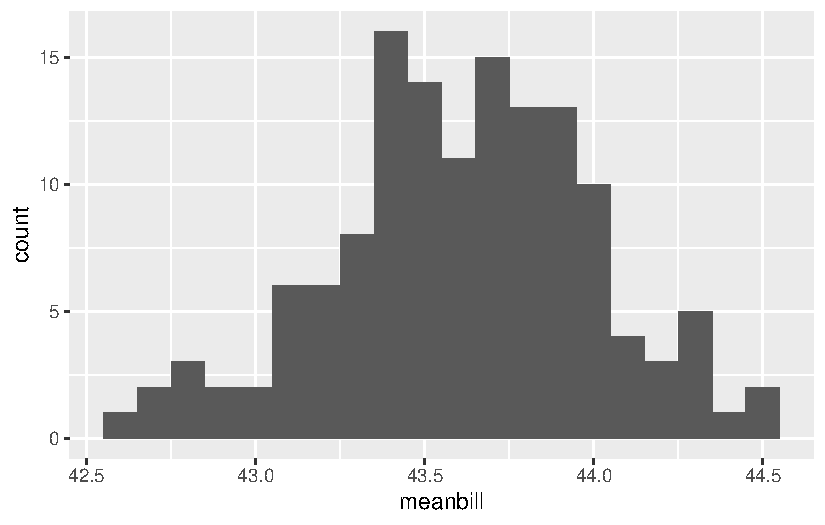
\includegraphics{CIs_files/figure-pdf/unnamed-chunk-7-1.pdf}

}

\end{figure}

\begin{Shaded}
\begin{Highlighting}[]
\CommentTok{\#check against original df}
\NormalTok{pen\_df\_bs}\OtherTok{\textless{}{-}} \DecValTok{1}\SpecialCharTok{:}\DecValTok{1000} \SpecialCharTok{\%\textgreater{}\%} \CommentTok{\#1000 = number of trials / resamples}
  \FunctionTok{map\_dfr}\NormalTok{(}
    \SpecialCharTok{\textasciitilde{}}\NormalTok{penguins }\SpecialCharTok{\%\textgreater{}\%}
      \FunctionTok{slice\_sample}\NormalTok{(}\AttributeTok{n=}\NormalTok{n, }\AttributeTok{replace=}\ConstantTok{TRUE}\NormalTok{) }\SpecialCharTok{\%\textgreater{}\%}
      \FunctionTok{summarize}\NormalTok{(}\AttributeTok{meanbill=}\FunctionTok{mean}\NormalTok{(bill\_length\_mm))) }\SpecialCharTok{\%\textgreater{}\%}
  \FunctionTok{mutate}\NormalTok{(}\AttributeTok{n=}\NormalTok{n)}

\NormalTok{pen\_df\_bs }
\end{Highlighting}
\end{Shaded}

\begin{verbatim}
# A tibble: 1,000 x 2
   meanbill     n
      <dbl> <dbl>
 1     NA     200
 2     NA     200
 3     NA     200
 4     NA     200
 5     NA     200
 6     44.1   200
 7     NA     200
 8     NA     200
 9     NA     200
10     NA     200
# i 990 more rows
\end{verbatim}

\begin{Shaded}
\begin{Highlighting}[]
\NormalTok{pen\_df\_bs }\SpecialCharTok{\%\textgreater{}\%}
  \FunctionTok{skim}\NormalTok{(meanbill) }\CommentTok{\#mean=44, sd=0.370}
\end{Highlighting}
\end{Shaded}

\begin{longtable}[]{@{}ll@{}}
\caption{Data summary}\tabularnewline
\toprule\noalign{}
\endfirsthead
\endhead
\bottomrule\noalign{}
\endlastfoot
Name & Piped data \\
Number of rows & 1000 \\
Number of columns & 2 \\
\_\_\_\_\_\_\_\_\_\_\_\_\_\_\_\_\_\_\_\_\_\_\_ & \\
Column type frequency: & \\
numeric & 1 \\
\_\_\_\_\_\_\_\_\_\_\_\_\_\_\_\_\_\_\_\_\_\_\_\_ & \\
Group variables & None \\
\end{longtable}

\textbf{Variable type: numeric}

\begin{longtable}[]{@{}
  >{\raggedright\arraybackslash}p{(\columnwidth - 20\tabcolsep) * \real{0.1647}}
  >{\raggedleft\arraybackslash}p{(\columnwidth - 20\tabcolsep) * \real{0.1176}}
  >{\raggedleft\arraybackslash}p{(\columnwidth - 20\tabcolsep) * \real{0.1647}}
  >{\raggedleft\arraybackslash}p{(\columnwidth - 20\tabcolsep) * \real{0.0706}}
  >{\raggedleft\arraybackslash}p{(\columnwidth - 20\tabcolsep) * \real{0.0588}}
  >{\raggedleft\arraybackslash}p{(\columnwidth - 20\tabcolsep) * \real{0.0706}}
  >{\raggedleft\arraybackslash}p{(\columnwidth - 20\tabcolsep) * \real{0.0706}}
  >{\raggedleft\arraybackslash}p{(\columnwidth - 20\tabcolsep) * \real{0.0706}}
  >{\raggedleft\arraybackslash}p{(\columnwidth - 20\tabcolsep) * \real{0.0706}}
  >{\raggedleft\arraybackslash}p{(\columnwidth - 20\tabcolsep) * \real{0.0706}}
  >{\raggedright\arraybackslash}p{(\columnwidth - 20\tabcolsep) * \real{0.0706}}@{}}
\toprule\noalign{}
\begin{minipage}[b]{\linewidth}\raggedright
skim\_variable
\end{minipage} & \begin{minipage}[b]{\linewidth}\raggedleft
n\_missing
\end{minipage} & \begin{minipage}[b]{\linewidth}\raggedleft
complete\_rate
\end{minipage} & \begin{minipage}[b]{\linewidth}\raggedleft
mean
\end{minipage} & \begin{minipage}[b]{\linewidth}\raggedleft
sd
\end{minipage} & \begin{minipage}[b]{\linewidth}\raggedleft
p0
\end{minipage} & \begin{minipage}[b]{\linewidth}\raggedleft
p25
\end{minipage} & \begin{minipage}[b]{\linewidth}\raggedleft
p50
\end{minipage} & \begin{minipage}[b]{\linewidth}\raggedleft
p75
\end{minipage} & \begin{minipage}[b]{\linewidth}\raggedleft
p100
\end{minipage} & \begin{minipage}[b]{\linewidth}\raggedright
hist
\end{minipage} \\
\midrule\noalign{}
\endhead
\bottomrule\noalign{}
\endlastfoot
meanbill & 685 & 0.31 & 43.88 & 0.38 & 42.94 & 43.63 & 43.88 & 44.14 &
44.97 & ▂▆▇▅▁ \\
\end{longtable}

\begin{Shaded}
\begin{Highlighting}[]
\CommentTok{\#histo}
\NormalTok{raw}\OtherTok{\textless{}{-}}\FunctionTok{ggplot}\NormalTok{(}\AttributeTok{data=}\NormalTok{pen\_df\_bs, }\FunctionTok{aes}\NormalTok{(}\AttributeTok{x=}\NormalTok{meanbill))}\SpecialCharTok{+}
  \FunctionTok{geom\_histogram}\NormalTok{(}\AttributeTok{binwidth=}\FloatTok{0.1}\NormalTok{)}
\NormalTok{raw}
\end{Highlighting}
\end{Shaded}

\begin{verbatim}
Warning: Removed 685 rows containing non-finite values (`stat_bin()`).
\end{verbatim}

\begin{figure}[H]

{\centering 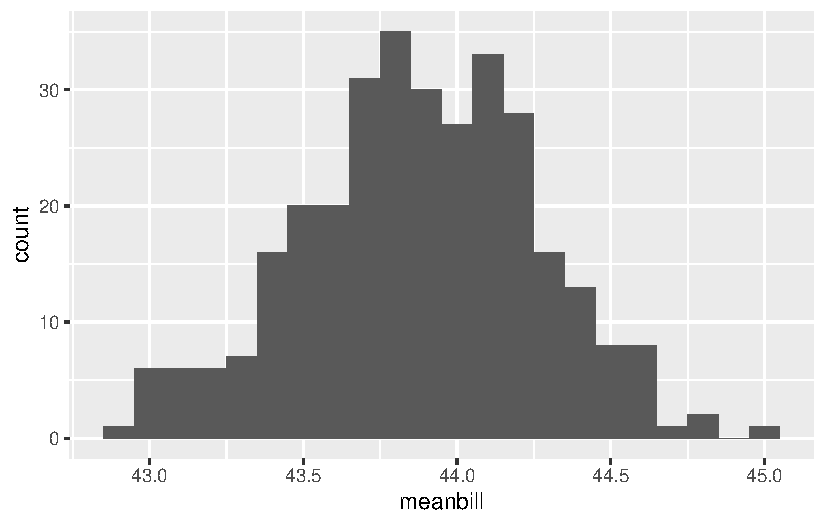
\includegraphics{CIs_files/figure-pdf/unnamed-chunk-7-2.pdf}

}

\end{figure}

\begin{Shaded}
\begin{Highlighting}[]
\CommentTok{\#compare:}
\NormalTok{raw}\SpecialCharTok{/}\NormalTok{bootplot}
\end{Highlighting}
\end{Shaded}

\begin{verbatim}
Warning: Removed 685 rows containing non-finite values (`stat_bin()`).
Removed 863 rows containing non-finite values (`stat_bin()`).
\end{verbatim}

\begin{figure}[H]

{\centering 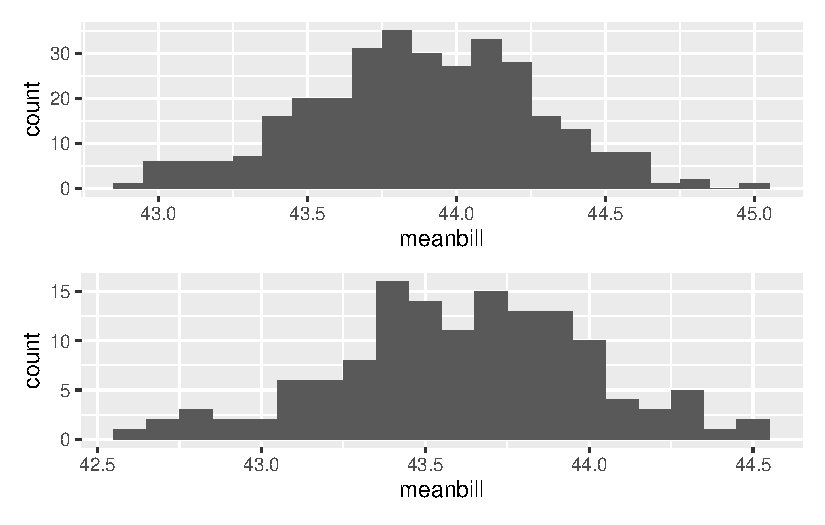
\includegraphics{CIs_files/figure-pdf/unnamed-chunk-7-3.pdf}

}

\end{figure}

-The distribution of values we get when we build a series of bootstrap
trials is called the bootstrap distribution. It is not exactly the same
as the sampling distribution but for sufficiently large n is is a good
approximation!

-Remember that if we have a roughly normal distribution we can get 95\%
CIs by using the rule of thump CI=2\emph{SE (or standard error of the
mean) \#the ``real'' value here is 1.96}SE

\hypertarget{calculating-boostrapped-cis-thus-could-look-like-this}{%
\subsection{calculating boostrapped CIs thus, could look like
this}\label{calculating-boostrapped-cis-thus-could-look-like-this}}

\begin{Shaded}
\begin{Highlighting}[]
\NormalTok{pen\_200\_bs}\OtherTok{\textless{}{-}} \DecValTok{1}\SpecialCharTok{:}\DecValTok{1000} \SpecialCharTok{\%\textgreater{}\%} \CommentTok{\#1000 = number of trials / resamples}
  \FunctionTok{map\_dfr}\NormalTok{(}
    \SpecialCharTok{\textasciitilde{}}\NormalTok{orig\_sample }\SpecialCharTok{\%\textgreater{}\%}
      \FunctionTok{slice\_sample}\NormalTok{(}\AttributeTok{n=}\NormalTok{n, }\AttributeTok{replace=}\ConstantTok{TRUE}\NormalTok{) }\SpecialCharTok{\%\textgreater{}\%}
      \FunctionTok{summarize}\NormalTok{(}\AttributeTok{meanbill=}\FunctionTok{mean}\NormalTok{(bill\_length\_mm))) }\SpecialCharTok{\%\textgreater{}\%}
  \FunctionTok{mutate}\NormalTok{(}\AttributeTok{n=}\NormalTok{n)}

\NormalTok{calc\_CIs}\OtherTok{\textless{}{-}}\NormalTok{pen\_200\_bs }\SpecialCharTok{\%\textgreater{}\%}
  \FunctionTok{summarize}\NormalTok{(}\AttributeTok{meanbillboot=}\FunctionTok{mean}\NormalTok{(meanbill), }\AttributeTok{CI=}\FloatTok{1.96}\SpecialCharTok{*}\FunctionTok{sd}\NormalTok{(meanbill))}

\NormalTok{calc\_CIs}
\end{Highlighting}
\end{Shaded}

\begin{verbatim}
# A tibble: 1 x 2
  meanbillboot    CI
         <dbl> <dbl>
1           NA    NA
\end{verbatim}

We did it!

\hypertarget{how-to-use-the-infer-package-to-do-cis}{%
\section{How to use the infer package to do
CIs!}\label{how-to-use-the-infer-package-to-do-cis}}

\begin{Shaded}
\begin{Highlighting}[]
\FunctionTok{library}\NormalTok{(infer)}
\end{Highlighting}
\end{Shaded}

\begin{verbatim}
Warning: package 'infer' was built under R version 4.2.3
\end{verbatim}

\begin{Shaded}
\begin{Highlighting}[]
\NormalTok{orig\_sample}
\end{Highlighting}
\end{Shaded}

\begin{verbatim}
# A tibble: 200 x 8
   species   island bill_length_mm bill_depth_mm flipper_length_mm body_mass_g
   <fct>     <fct>           <dbl>         <dbl>             <int>       <int>
 1 Adelie    Biscoe           39.7          17.7               193        3200
 2 Gentoo    Biscoe           47.5          14                 212        4875
 3 Chinstrap Dream            50.5          18.4               200        3400
 4 Gentoo    Biscoe           46.6          14.2               210        4850
 5 Chinstrap Dream            46.6          17.8               193        3800
 6 Adelie    Dream            40.3          18.5               196        4350
 7 Gentoo    Biscoe           45.1          14.4               210        4400
 8 Adelie    Biscoe           35.3          18.9               187        3800
 9 Gentoo    Biscoe           45.1          14.5               207        5050
10 Gentoo    Biscoe           42.9          13.1               215        5000
# i 190 more rows
# i 2 more variables: sex <fct>, year <int>
\end{verbatim}

\begin{Shaded}
\begin{Highlighting}[]
\CommentTok{\#dplyr method for mean}
\NormalTok{orig\_sample }\SpecialCharTok{\%\textgreater{}\%}
  \FunctionTok{summarize}\NormalTok{(}\AttributeTok{stat=}\FunctionTok{mean}\NormalTok{(bill\_length\_mm))}
\end{Highlighting}
\end{Shaded}

\begin{verbatim}
# A tibble: 1 x 1
   stat
  <dbl>
1    NA
\end{verbatim}

\begin{Shaded}
\begin{Highlighting}[]
\CommentTok{\#44.0}
\NormalTok{x\_bar}\OtherTok{=}\FloatTok{44.0}


\CommentTok{\#infer method for mean}
\NormalTok{orig\_sample }\SpecialCharTok{\%\textgreater{}\%}
  \FunctionTok{specify}\NormalTok{(}\AttributeTok{response =}\NormalTok{ bill\_length\_mm) }\SpecialCharTok{\%\textgreater{}\%}
  \FunctionTok{calculate}\NormalTok{(}\AttributeTok{stat=}\StringTok{\textquotesingle{}mean\textquotesingle{}}\NormalTok{)}
\end{Highlighting}
\end{Shaded}

\begin{verbatim}
Warning: Removed 2 rows containing missing values.
\end{verbatim}

\begin{verbatim}
Response: bill_length_mm (numeric)
# A tibble: 1 x 1
   stat
  <dbl>
1  43.6
\end{verbatim}

\begin{Shaded}
\begin{Highlighting}[]
\CommentTok{\#make bootstrap distribution }
\NormalTok{boot\_dist }\OtherTok{\textless{}{-}}\NormalTok{orig\_sample }\SpecialCharTok{\%\textgreater{}\%}
  \FunctionTok{specify}\NormalTok{(}\AttributeTok{response=}\NormalTok{bill\_length\_mm) }\SpecialCharTok{\%\textgreater{}\%}
  \FunctionTok{generate}\NormalTok{(}\AttributeTok{reps=}\DecValTok{1000}\NormalTok{) }\SpecialCharTok{\%\textgreater{}\%}
  \FunctionTok{calculate}\NormalTok{(}\AttributeTok{stat=}\StringTok{\textquotesingle{}mean\textquotesingle{}}\NormalTok{)}
\end{Highlighting}
\end{Shaded}

\begin{verbatim}
Warning: Removed 2 rows containing missing values.
\end{verbatim}

\begin{verbatim}
Setting `type = "bootstrap"` in `generate()`.
\end{verbatim}

\begin{Shaded}
\begin{Highlighting}[]
\NormalTok{boot\_dist}
\end{Highlighting}
\end{Shaded}

\begin{verbatim}
Response: bill_length_mm (numeric)
# A tibble: 1,000 x 2
   replicate  stat
       <int> <dbl>
 1         1  43.9
 2         2  43.2
 3         3  43.8
 4         4  43.0
 5         5  43.6
 6         6  43.9
 7         7  44.2
 8         8  43.9
 9         9  42.6
10        10  43.6
# i 990 more rows
\end{verbatim}

\begin{Shaded}
\begin{Highlighting}[]
\CommentTok{\#look at the histo}
\FunctionTok{visualize}\NormalTok{(boot\_dist)}
\end{Highlighting}
\end{Shaded}

\begin{figure}[H]

{\centering 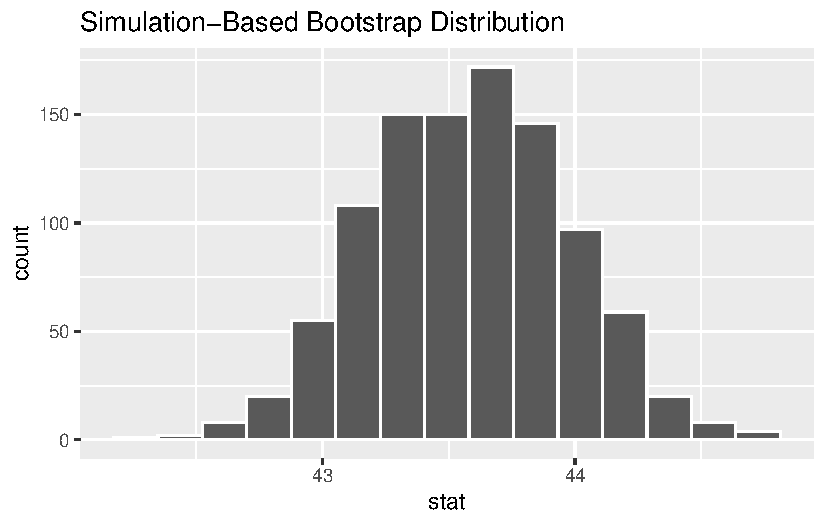
\includegraphics{CIs_files/figure-pdf/unnamed-chunk-9-1.pdf}

}

\end{figure}

\begin{Shaded}
\begin{Highlighting}[]
\CommentTok{\#percentile based CIs}
\NormalTok{percentile\_ci }\OtherTok{\textless{}{-}}\NormalTok{ boot\_dist }\SpecialCharTok{\%\textgreater{}\%} 
  \FunctionTok{get\_confidence\_interval}\NormalTok{(}\AttributeTok{level =} \FloatTok{0.95}\NormalTok{, }\AttributeTok{type =} \StringTok{"percentile"}\NormalTok{)}

\NormalTok{percentile\_ci}
\end{Highlighting}
\end{Shaded}

\begin{verbatim}
# A tibble: 1 x 2
  lower_ci upper_ci
     <dbl>    <dbl>
1     42.9     44.3
\end{verbatim}

\begin{Shaded}
\begin{Highlighting}[]
\CommentTok{\#graphically....}
\FunctionTok{visualize}\NormalTok{(boot\_dist) }\SpecialCharTok{+} 
  \FunctionTok{shade\_confidence\_interval}\NormalTok{(}\AttributeTok{endpoints =}\NormalTok{ percentile\_ci)}
\end{Highlighting}
\end{Shaded}

\begin{figure}[H]

{\centering 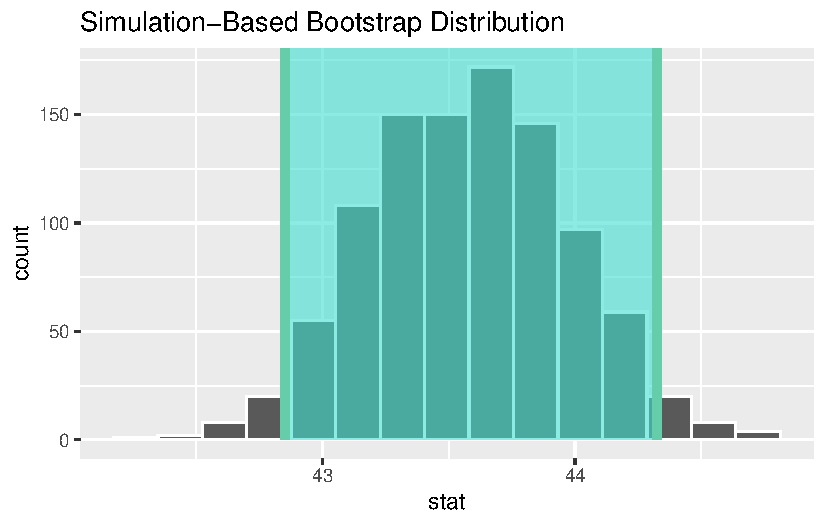
\includegraphics{CIs_files/figure-pdf/unnamed-chunk-9-2.pdf}

}

\end{figure}

\begin{Shaded}
\begin{Highlighting}[]
\CommentTok{\#CIs via standard error}
\NormalTok{se\_CI}\OtherTok{\textless{}{-}}\NormalTok{ boot\_dist }\SpecialCharTok{\%\textgreater{}\%}
  \FunctionTok{get\_confidence\_interval}\NormalTok{(}\AttributeTok{type=}\StringTok{\textquotesingle{}se\textquotesingle{}}\NormalTok{, }\AttributeTok{point\_estimate =}\NormalTok{ x\_bar) }\CommentTok{\#where x\_bar is the original sample mean}
\end{Highlighting}
\end{Shaded}

\begin{verbatim}
Using `level = 0.95` to compute confidence interval.
\end{verbatim}

\begin{Shaded}
\begin{Highlighting}[]
\NormalTok{se\_CI}
\end{Highlighting}
\end{Shaded}

\begin{verbatim}
# A tibble: 1 x 2
  lower_ci upper_ci
     <dbl>    <dbl>
1     43.2     44.8
\end{verbatim}

\begin{Shaded}
\begin{Highlighting}[]
\DocumentationTok{\#\#\# let\textquotesingle{}s see how the CI values line up: }
\NormalTok{calc\_CIs}
\end{Highlighting}
\end{Shaded}

\begin{verbatim}
# A tibble: 1 x 2
  meanbillboot    CI
         <dbl> <dbl>
1           NA    NA
\end{verbatim}

\begin{Shaded}
\begin{Highlighting}[]
\DecValTok{44}\FloatTok{{-}0.783} \CommentTok{\#43.217}
\end{Highlighting}
\end{Shaded}

\begin{verbatim}
[1] 43.217
\end{verbatim}

\begin{Shaded}
\begin{Highlighting}[]
\DecValTok{44}\FloatTok{+0.783} \CommentTok{\#44.783}
\end{Highlighting}
\end{Shaded}

\begin{verbatim}
[1] 44.783
\end{verbatim}

\begin{Shaded}
\begin{Highlighting}[]
\NormalTok{percentile\_ci }\CommentTok{\#43.2, 44.8}
\end{Highlighting}
\end{Shaded}

\begin{verbatim}
# A tibble: 1 x 2
  lower_ci upper_ci
     <dbl>    <dbl>
1     42.9     44.3
\end{verbatim}

\begin{Shaded}
\begin{Highlighting}[]
\NormalTok{se\_CI }\CommentTok{\# 43.2, 44.8}
\end{Highlighting}
\end{Shaded}

\begin{verbatim}
# A tibble: 1 x 2
  lower_ci upper_ci
     <dbl>    <dbl>
1     43.2     44.8
\end{verbatim}

\begin{Shaded}
\begin{Highlighting}[]
\CommentTok{\#all super close!}
\end{Highlighting}
\end{Shaded}




\end{document}
